\documentclass[11pt,a4paper]{article}

\usepackage[utf8]{inputenc}
\usepackage[T1]{fontenc}
\usepackage[margin=2.5cm]{geometry}
\usepackage{amsmath,amssymb,bm}
\usepackage{booktabs}
\usepackage{array}
\usepackage{enumerate}
\usepackage{xcolor}
\usepackage{hyperref}
\usepackage{tikz}

\hypersetup{colorlinks=true, linkcolor=blue, urlcolor=blue}

\newcommand{\points}[1]{\textbf{(#1\,\%)}}
\newcommand{\subpoints}[1]{\textit{(#1\,\%)}}

\title{TMA4268 Statistical Learning V2026\\[0.3em]
\large Mock Exam 1 (estimated final exam)}
\author{Compiled by Claude for Anders Bekkevard\\[0.2em]
\small Based on the Apr 28 exam-review lecture, the 2023--2025 finals, and the prof's stated scope rule}
\date{Mock for: May 18, 2026 (real exam date)}

\begin{document}
\maketitle

\noindent\fbox{\parbox{\dimexpr\textwidth-2\fboxsep-2\fboxrule}{%
\textbf{Instructions.}
\begin{itemize}
  \item \textbf{Duration:} 4 hours. \textbf{Open book.} Permitted aids: ISLP (2nd ed.), one handwritten A5 sheet of notes, calculator.
  \item \textbf{No code required.} Write answers as math, plain English, or pseudocode. Do \emph{not} memorize R/Python package names.
  \item \textbf{Show your work} --- partial credit is generously available, including when calculator slips spoil a numeric answer but the setup is correct.
  \item \textbf{No negative scoring.} Always answer, even when unsure.
  \item \textbf{If a question seems broken or ambiguous}, state the assumption you are making in one short sentence and proceed.
  \item Total: \textbf{100 points = 100\,\%}. Per-problem weights given in parentheses.
\end{itemize}}}

\vspace{0.6em}
\noindent\textbf{Grade boundaries (NTNU \emph{prosentvurderingsmetoden}, advisory):}
A: 89--100\,\% \quad B: 77--88\,\% \quad C: 65--76\,\% \quad D: 53--64\,\% \quad E: 41--52\,\% \quad F: 0--40\,\%.

\vspace{1em}
\hrule
\vspace{1em}

%=========================================================
\section*{Problem 1 \points{10} --- Fill-in-the-blank concepts}
%=========================================================

\noindent Read the passage and pick the best word for each blank from the choices in parentheses. Each correct fill is worth $1$\,\%.

\bigskip

In this course we studied methods that learn from data. Our methods were broadly divided into \underline{\hspace{2cm}}\,(1) (\emph{supervised} / \emph{unsupervised} / \emph{parametric} / \emph{deterministic}) and unsupervised learning. In the supervised setting we distinguished problems with a quantitative response (regression) from problems with a qualitative response (\underline{\hspace{2cm}}\,(2) (\emph{clustering} / \emph{classification} / \emph{dimensionality reduction})).

We also separated two motivations: when we care mostly about the actual coefficients of the fitted model and what they mean, we are doing \underline{\hspace{2cm}}\,(3) (\emph{prediction} / \emph{inference} / \emph{interpolation} / \emph{regularization}). When we instead only care about $\hat y$ being close to the true $y$ on unseen data, we are doing \underline{\hspace{2cm}}\,(4) (\emph{prediction} / \emph{inference} / \emph{cross-validation} / \emph{shrinkage}).

A central theme of the course was the bias--variance decomposition. The expected squared test error at a fixed point $x_0$ splits into three pieces: a squared-bias term, a variance term, and an \underline{\hspace{2cm}}\,(5) (\emph{irreducible} / \emph{reducible} / \emph{biased} / \emph{averaged}) error. Methods that explicitly trade a little extra bias for a large reduction in variance are called \underline{\hspace{2cm}}\,(6) (\emph{regularization methods} / \emph{boosted methods} / \emph{generative methods} / \emph{bootstrap methods}).

For classification we discussed both \emph{generative} approaches (which model $P(X \mid Y\!=\!k)$ and the class priors) and \emph{discriminative} approaches (which model $P(Y \mid X)$ directly). Among the methods we studied, \underline{\hspace{2cm}}\,(7) (\emph{logistic regression} / \emph{LDA} / \emph{KNN} / \emph{ridge regression}) belongs to the discriminative family, while LDA and QDA are \underline{\hspace{2cm}}\,(8) (\emph{generative} / \emph{nonparametric} / \emph{distance-based}).

Finally, in unsupervised learning we studied \underline{\hspace{2cm}}\,(9) (\emph{principal component analysis} / \emph{ridge regression} / \emph{the bootstrap}) as a linear dimensionality-reduction tool, and clustering methods such as $K$-means and \underline{\hspace{2cm}}\,(10) (\emph{hierarchical clustering} / \emph{logistic clustering} / \emph{kernel PCA}).

\vfill\eject

%=========================================================
\section*{Problem 2 \points{28} --- Multiple choice, true/false, and short numeric}
%=========================================================

For each subproblem, write \emph{True/False} for each statement (or the requested numeric answer). For true/false subproblems, you may add a one-sentence justification but only if you think it helps; do not write essays.

\subsection*{a) Bias--variance reasoning \subpoints{3}}
Which of the following statements are true?
\begin{enumerate}[(i)]
  \item As the flexibility of a fitted model increases, its squared bias generally decreases.
  \item As the flexibility of a fitted model increases, its variance generally decreases.
  \item In a high-noise (large $\sigma^2$) setting, a very flexible model is generally preferable to a less flexible one.
  \item The irreducible error $\sigma^2$ can be driven arbitrarily close to zero by collecting more training data.
\end{enumerate}

\subsection*{b) Ridge vs.\ Lasso \subpoints{3}}
Which of the following are true?
\begin{enumerate}[(i)]
  \item Increasing the penalty parameter $\lambda$ in ridge regression shrinks coefficients toward zero but, for any finite $\lambda$, never makes any coefficient exactly zero.
  \item Lasso can produce sparse models because the $\ell_1$ penalty ball has corners on the coordinate axes.
  \item Ridge regression is more flexible than ordinary least squares.
  \item Standardizing the predictors before fitting ridge or lasso is generally recommended.
\end{enumerate}

\subsection*{c) Neural network parameters and forward pass \subpoints{4}}
Suppose you build a fully-connected feed-forward neural network with:
\begin{itemize}
  \item $5$ input variables,
  \item one hidden layer of $6$ neurons (with bias),
  \item one output neuron (with bias).
\end{itemize}

\begin{enumerate}[(i)]
  \item \subpoints{2} How many weights (parameters) does the network have in total, \emph{including bias terms}?
  \item \subpoints{2} A neuron in the hidden layer has weights $w_1 = 0.5,\, w_2 = -1.0,\, w_3 = 0.0,\, w_4 = 2.0,\, w_5 = -0.5$ and bias $b = 0.3$. Its inputs on a given observation are $x_1 = 2,\, x_2 = 1,\, x_3 = -3,\, x_4 = 0.5,\, x_5 = 4$. Using a ReLU activation, what is the output of this neuron?
\end{enumerate}

\subsection*{d) Odds and probability \subpoints{3}}
\begin{enumerate}[(i)]
  \item \subpoints{1} A study reports that the odds of an event are $2.5$. What is the probability of the event?
  \item \subpoints{1} An individual has a $30\%$ probability of defaulting on her credit card. What are her odds of defaulting?
  \item \subpoints{1} In a logistic-regression fit, the coefficient on a binary predictor $D$ (smoker = $1$, non-smoker = $0$) equals $\hat\beta = 0.8$. By what factor do the odds of the response event change for a smoker relative to a non-smoker, holding all other predictors fixed? (One numeric value.)
\end{enumerate}

\subsection*{e) Smoothing splines and degrees of freedom \subpoints{3}}
Consider a smoothing spline fit with smoothing parameter $\lambda$.

Which of the following are true?
\begin{enumerate}[(i)]
  \item As $\lambda \to 0$, the fit approaches the rough interpolating spline that passes through every training point.
  \item As $\lambda \to \infty$, the fit approaches the ordinary-least-squares straight line.
  \item Increasing $\lambda$ \emph{increases} the effective degrees of freedom of the fit.
  \item The effective degrees of freedom $\mathrm{df}_\lambda = \mathrm{tr}(S_\lambda)$ of a smoothing spline is, in general, not an integer.
\end{enumerate}

\subsection*{f) Principal component analysis \subpoints{5}}
You perform PCA on a dataset with six \textbf{standardized} variables $X_1, \dots, X_6$ and obtain:
\begin{center}\small
\begin{tabular}{lcc}
\toprule
\textbf{PC} & \textbf{Eigenvalue} & \textbf{PVE} \\
\midrule
PC1 & 2.4 & 0.40 \\
PC2 & 1.5 & 0.25 \\
PC3 & 1.2 & 0.20 \\
PC4 & 0.5 & $\approx$0.083 \\
PC5 & 0.3 & 0.05 \\
PC6 & 0.1 & $\approx$0.017 \\
\bottomrule
\end{tabular}
\end{center}

The loading vector of the first principal component (entries rounded to two decimal places) is
$$\phi_1 = (\,0.60,\; 0.50,\; 0.40,\; 0.30,\; 0.30,\; 0.20\,)^\top.$$
A new observation has standardized values
$$x^* = (\,1,\; -1,\; 0.5,\; 2,\; 0,\; -1\,)^\top.$$

\begin{enumerate}[(i)]
  \item \subpoints{1} What is the total variance in the standardized data?
  \item \subpoints{1} What proportion of the total variance is explained by PC1 and PC2 together?
  \item \subpoints{1} How many principal components must be kept to retain at least $85\%$ of the total variance?
  \item \subpoints{1} Compute the score $z^*_1$ of the new observation on PC1.
  \item \subpoints{1} Which one variable contributes \emph{most} to PC1?
\end{enumerate}

\subsection*{g) Sensitivity, specificity, ROC, and AUC \subpoints{3}}
A classifier is applied to a test set of $1000$ patients, of whom $200$ truly have the disease. At a chosen threshold the confusion matrix is:
\begin{center}\small
\begin{tabular}{c|cc}
 & \textbf{Predicted: disease} & \textbf{Predicted: no disease} \\ \hline
\textbf{Actual: disease}    & 140 & 60 \\
\textbf{Actual: no disease} & 80  & 720 \\
\end{tabular}
\end{center}

\begin{enumerate}[(i)]
  \item \subpoints{1} Compute the \emph{sensitivity} of the classifier.
  \item \subpoints{1} Compute the \emph{specificity} of the classifier.
  \item \subpoints{1} Which of the following is true about the AUC (area under the ROC curve)? Mark all that apply.
  \begin{itemize}
    \item[(A)] AUC $= 0.5$ corresponds to a classifier no better than random guessing.
    \item[(B)] Two classifiers with the same AUC must produce ROC curves of the same shape.
    \item[(C)] The ROC curve plots true positive rate (TPR) on the $y$-axis against false positive rate (FPR) on the $x$-axis, varying the classification threshold.
    \item[(D)] AUC is unaffected by class imbalance in the way raw accuracy is.
  \end{itemize}
\end{enumerate}

\subsection*{h) Why are nonlinear activations necessary? \subpoints{2}}
Mark all that are true. In a feed-forward neural network, the hidden-layer activation function is nonlinear because\dots
\begin{enumerate}[(i)]
  \item it allows the network to approximate complex, non-linear functions of the inputs;
  \item without it the entire network collapses to an affine map of the input, no matter how many hidden layers are stacked;
  \item it acts as an implicit regularizer that shrinks the hidden weights toward zero;
  \item it makes the empirical loss surface convex in the network weights.
\end{enumerate}

\subsection*{i) LDA vs.\ QDA \subpoints{2}}
Mark all that are true.
\begin{enumerate}[(i)]
  \item LDA assumes a single shared within-class covariance matrix $\Sigma$, whereas QDA allows a separate $\Sigma_k$ for each class.
  \item Under LDA's assumption, the resulting Bayes decision boundary is \emph{linear} in the features because the quadratic term $\mathbf{x}^\top \Sigma^{-1} \mathbf{x}$ is identical for every class and therefore cancels when discriminant functions are compared.
  \item In a regime with very few training observations per class, QDA generally outperforms LDA because QDA is more flexible.
  \item LDA and QDA are both \emph{generative} classifiers: they model $P(\mathbf{X}\mid Y\!=\!k)$ and the class priors $\pi_k$ and then apply Bayes' rule.
\end{enumerate}

\vfill\eject

%=========================================================
\section*{Problem 3 \points{16} --- Theory and hand calculations}
%=========================================================

\subsection*{a) The mathy one --- maximum likelihood and least squares \subpoints{8}}

Consider a regression setting in which the response is modelled as
$$Y_i = f_\theta(X_i) + \varepsilon_i, \qquad i = 1,\dots,n,$$
where $f_\theta$ is a regression function indexed by an unknown parameter vector $\theta$, the inputs $X_i$ are treated as fixed, and the errors $\varepsilon_i$ are independent and identically distributed (i.i.d.).

\begin{enumerate}[(i)]
  \item \subpoints{2} Write down the optimization problem that defines the \emph{ordinary least-squares} estimator $\hat\theta_{\mathrm{LS}}$ of $\theta$. State the minimal assumptions on $\varepsilon_i$ needed for this estimator to be well-defined.
  \item \subpoints{2} Now additionally assume $\varepsilon_i \sim \mathcal{N}(0, \sigma^2)$. Write down the log-likelihood $\ell(\theta, \sigma^2)$ of the sample $(Y_1,\dots,Y_n)$.
  \item \subpoints{3} Show that the maximum-likelihood estimator $\hat\theta_{\mathrm{MLE}}$ and the least-squares estimator $\hat\theta_{\mathrm{LS}}$ \emph{coincide} under the Gaussian-error assumption. Be explicit about which terms in your log-likelihood do and do not depend on $\theta$.
  \item \subpoints{1} Does this equivalence still hold if you replace the Gaussian assumption with $\varepsilon_i \sim \mathrm{Laplace}(0, b)$? Briefly justify your answer (one or two sentences).
\end{enumerate}

\subsection*{b) Hierarchical clustering by hand \subpoints{5}}

Four observations have the following Euclidean dissimilarity matrix:
$$D = \begin{pmatrix}
0 & 4 & 9 & 8 \\
4 & 0 & 5 & 6 \\
9 & 5 & 0 & 3 \\
8 & 6 & 3 & 0 \\
\end{pmatrix}.$$

\begin{enumerate}[(i)]
  \item \subpoints{3} Sketch the dendrogram produced by hierarchical clustering with \emph{complete} linkage. Label the leaves $1, 2, 3, 4$, indicate the fusion height of each merge on a properly labelled $y$-axis, and show the recomputed dissimilarity matrix after the first merge.
  \item \subpoints{1} If instead you use \emph{single} linkage on the same matrix, what would change about the \emph{first} merge? Justify in one sentence.
  \item \subpoints{1} Suppose you cut the complete-linkage dendrogram at height $7$. How many clusters do you obtain, and which observations are in each cluster?
\end{enumerate}

\subsection*{c) The bias--variance decomposition \subpoints{3}}

\begin{enumerate}[(i)]
  \item \subpoints{2} Let $y_0 = f(x_0) + \varepsilon$ with $\mathbb{E}[\varepsilon] = 0$ and $\mathrm{Var}(\varepsilon) = \sigma^2$, and let $\hat f$ be a model fit on a random training set, with $\hat f$ independent of $\varepsilon$. Write down the bias--variance decomposition of the expected squared test error $\mathbb{E}\!\left[(y_0 - \hat f(x_0))^2\right]$ as a sum of three terms. \emph{Identify each term by name} and \emph{state what the expectations are taken over}.
  \item \subpoints{1} In one or two sentences, give a reason why one might prefer the label \emph{bias--variance decomposition} over \emph{bias--variance trade-off}. (You may, for example, appeal to the squared form of the bias term, the role of a clever model choice such as regularization, or the over-parameterized regime in which both bias and variance can simultaneously decrease.)
\end{enumerate}

\vfill\eject

%=========================================================
\section*{Problem 4 \points{22} --- Data analysis: regression on used-car prices}
%=========================================================

A dealership records $n = 500$ used-car transactions. The response is the sale \texttt{price} (in $1000$ EUR). The available predictors are:
\begin{itemize}
  \item \texttt{mileage} --- total mileage in $1000$ km (continuous);
  \item \texttt{age} --- age of the car in years (continuous);
  \item \texttt{horsepower} --- engine power, hp (continuous);
  \item \texttt{engine} --- engine displacement, litres (continuous);
  \item \texttt{mpg} --- combined fuel economy (continuous);
  \item \texttt{fuel} --- categorical: \emph{petrol} (reference), \emph{diesel}, \emph{electric}.
\end{itemize}

The course staff fit the linear model
$$\texttt{price} \sim \texttt{mileage} + \texttt{age} + I(\texttt{age}^2) + \texttt{horsepower} + \texttt{engine} + \texttt{mpg} + \texttt{fuel}$$
on a training set ($n_\text{train} = 350$, the remaining $150$ cars form the test set). The output is:

\begin{center}\small
\begin{tabular}{lcccc}
\toprule
 & \textbf{Estimate} & \textbf{Std.\ Error} & \textbf{t-value} & \textbf{Pr($>|t|$)} \\
\midrule
(Intercept)    & $24.50$  & $2.30$    & $10.65$  & $<0.001$ \\
\texttt{mileage}        & $-0.085$ & $0.012$   & $-7.08$  & $<0.001$ \\
\texttt{age}            & $-1.20$  & $0.40$    & $-3.00$  & $0.003$ \\
$I(\texttt{age}^2)$     & $0.030$  & $0.020$   & $1.50$   & $0.135$ \\
\texttt{horsepower}     & $0.045$  & $0.011$   & $4.09$   & $<0.001$ \\
\texttt{engine}         & $1.80$   & $0.65$    & $2.77$   & $0.006$ \\
\texttt{mpg}            & $0.12$   & $0.08$    & $1.50$   & $0.135$ \\
\texttt{fuel\_diesel}   & $-0.65$  & $0.55$    & $-1.18$  & $0.239$ \\
\texttt{fuel\_electric} & $3.20$   & $1.10$    & $2.91$   & $0.004$ \\
\bottomrule
\end{tabular}
\end{center}

\noindent Residual standard error: $2.10$ on $341$ degrees of freedom.\quad
Multiple $R^2 = 0.621$,\ Adjusted $R^2 = 0.612$.\quad
$F$-statistic on the categorical \texttt{fuel} variable (joint test of both dummies against \texttt{fuel = petrol}): $F = 4.85$ on $(2, 341)$ d.f., $p = 0.008$.

\subsection*{a) Reading the table \subpoints{6}}
\begin{enumerate}[(i)]
  \item \subpoints{1} How many parameters does this model estimate? (i.e.\ how many degrees of freedom does the model consume, including the intercept?) Justify your count briefly.
  \item \subpoints{2} An electric car is, on average, how much more or less expensive than an otherwise identical petrol car? Quantify both the point estimate and an approximate $95\%$ confidence interval (you may use $1.96$ as the critical value).
  \item \subpoints{2} Is there evidence that the categorical variable \texttt{fuel} is \emph{jointly} associated with \texttt{price}, after controlling for the other predictors? \textbf{Name the test you would use} and state your conclusion based on the output above. (You do \emph{not} need to compute the test statistic by hand.)
  \item \subpoints{1} A friend reads the table and concludes: ``\texttt{mpg} is irrelevant to the price.'' Briefly say in what sense she is right and in what sense she may be wrong (one or two sentences).
\end{enumerate}

\subsection*{b) Training vs.\ test error: the keyword \subpoints{3}}
Suppose you fit a second model that uses the same predictors as above but \emph{also} adds the cubic term $I(\texttt{age}^3)$ and the redundant term $I(\texttt{age}/12)$ (i.e.\ \texttt{age} re-expressed in different units).

\begin{enumerate}[(i)]
  \item \subpoints{1} Will the \emph{training} RSS of the larger model be lower than, equal to, or higher than that of the smaller model? Justify.
  \item \subpoints{1} What about the \emph{test} RSS? Can you be certain about the direction? Justify.
  \item \subpoints{1} What problem does the redundant term $I(\texttt{age}/12)$ create at fitting time, and what would happen if you added an $\ell_2$ penalty?
\end{enumerate}

\subsection*{c) Lasso with $10$-fold cross-validation \subpoints{6}}
The same predictors are now fed into a lasso regression. A $10$-fold cross-validation gives the following profile of CV-MSE against $\log \lambda$:

\begin{center}
\begin{tikzpicture}[scale=0.85]
  \draw[->] (0,0) -- (8.3,0) node[right] {$\log\lambda$};
  \draw[->] (0,0) -- (0,6.3) node[above] {CV-MSE};

  \draw[smooth, thick, blue] plot[domain=0.4:7.5] (\x, {2.5 + 0.03*(\x-1)*(\x-1) + 0.002*(\x-1)*(\x-1)*(\x-1)});

  \draw[dashed] (1,0) -- (1,5.6);
  \node[above] at (1,5.6) {\small $\hat\lambda_{\min}$};
  \draw[dashed] (3,0) -- (3,5.6);
  \node[above] at (3,5.6) {\small $\hat\lambda_{1\mathrm{SE}}$};

  \foreach \x in {0,2,4,6}
    \draw (\x, 0.06) -- (\x, -0.06) node[below] {\x};
  \foreach \y in {0,1,2,3,4,5,6}
    \draw (-0.06, \y) -- (0.06, \y) node[left,xshift=-0.1cm] {\y};

  \node[blue] at (6.3,4.6) {\small CV curve};
\end{tikzpicture}
\end{center}

\noindent (You may assume that the prediction-test MSEs you would obtain if you fitted the lasso at $\hat\lambda_{\min}$ and at $\hat\lambda_{1SE}$ are $5.20$ and $5.55$ respectively. The unregularized OLS model from part (a), evaluated on the same test set, gives test MSE $5.15$.)

\begin{enumerate}[(i)]
  \item \subpoints{1} Write down, in math or pseudocode, how the $10$-fold CV-MSE estimate at a fixed $\lambda$ is computed.
  \item \subpoints{1} Which value of $\lambda$ would you pick from the plot, and why? (Either $\hat\lambda_{\min}$ or $\hat\lambda_{1SE}$ is acceptable, but justify.)
  \item \subpoints{2} Compare the test MSE of the lasso (at $\hat\lambda_{\min}$) to the test MSE of OLS. Interpret the result in bias--variance terms: what does it tell you about the predictors in this dataset?
  \item \subpoints{2} On the plot above, the vertical dashed lines mark $\hat\lambda_{\min}$ (the $\lambda$ with the smallest CV error) and $\hat\lambda_{1\text{SE}}$ (the largest $\lambda$ whose CV error is within one standard error of the minimum). Briefly state the \emph{one-standard-error rule} and explain when a practitioner might prefer $\hat\lambda_{1\text{SE}}$ over $\hat\lambda_{\min}$.
\end{enumerate}

\subsection*{d) Tree boosting \subpoints{5}}

The same training set is now fit with a gradient-boosted tree model, evaluated on the same test set. The resulting test MSE is $3.85$, lower than the OLS and lasso test MSEs.

\begin{enumerate}[(i)]
  \item \subpoints{2} Gradient boosting has three main hyperparameters: the number of trees $B$, the interaction depth $d$, and the shrinkage (learning rate) $\eta$. For each, briefly say how you would choose its value and how it affects the bias--variance behaviour of the final model.
  \item \subpoints{1} Why is it incorrect to claim that $B$ ``does not matter as long as it is large enough''? (One sentence.)
  \item \subpoints{2} What does the lower test MSE of boosting compared to OLS suggest about the structure of the relationship between the predictors and \texttt{price}? What would you check next if you also wanted \emph{interpretation}, not just prediction?
\end{enumerate}

\subsection*{e) GAM degrees of freedom \subpoints{2}}
Finally, you fit a generalized additive model (GAM) of the form
$$\texttt{price} = \beta_0 + f_1(\texttt{mileage}) + f_2(\texttt{age}) + f_3(\texttt{horsepower}) + \beta_4 \cdot \texttt{engine} + \beta_5 \cdot \texttt{mpg} + g(\texttt{fuel}) + \varepsilon,$$
where $f_1, f_2, f_3$ are cubic regression splines, each with $4$ internal knots (and an intercept absorbed into $\beta_0$). The categorical \texttt{fuel} term $g(\texttt{fuel})$ uses dummy coding as in part (a).

\begin{enumerate}[(i)]
  \item \subpoints{1} How many degrees of freedom does the spline $f_1(\texttt{mileage})$ alone consume? (Count basis functions, excluding the global intercept.)
  \item \subpoints{1} How many total degrees of freedom does the GAM consume (including the intercept)?
\end{enumerate}

\vfill\eject

%=========================================================
\section*{Problem 5 \points{24} --- Data analysis: classification of loan defaults}
%=========================================================

A bank has data on $n = 10{,}000$ customers; the response \texttt{default} is binary ($1$ if the customer defaulted within the year, $0$ otherwise). Predictors include:
\begin{itemize}
  \item \texttt{balance} --- average outstanding monthly balance, in $1000$ EUR;
  \item \texttt{income} --- annual income, in $1000$ EUR;
  \item \texttt{sex} --- categorical: \emph{male} (reference), \emph{female};
  \item six payment-history variables \texttt{pay\_0}, \dots, \texttt{pay\_5}.
\end{itemize}

The data are split $70/30$ into a training set ($7000$) and a test set ($3000$).

\subsection*{a) Logistic regression with interaction \subpoints{10}}

A logistic regression model is fit on the training set, using all predictors plus the interaction \texttt{balance:sex}. The coefficient table for the most important rows is:

\begin{center}\small
\begin{tabular}{lcccc}
\toprule
 & \textbf{Estimate} & \textbf{Std.\ Error} & \textbf{z-value} & \textbf{Pr($>|z|$)} \\
\midrule
(Intercept)             & $-10.80$  & $0.45$     & $-24.0$ & $<0.001$ \\
\texttt{balance}        & $1.00$    & $0.05$     & $20.0$  & $<0.001$ \\
\texttt{income}         & $-0.010$  & $0.0025$   & $-4.0$  & $<0.001$ \\
\texttt{sex\_female}    & $-0.18$   & $0.35$     & $-0.51$ & $0.610$  \\
\texttt{balance:sex\_female} & $0.25$ & $0.08$  & $3.13$  & $0.002$  \\
\midrule
\texttt{pay\_0}         & $0.55$    & $0.04$     & $13.8$  & $<0.001$ \\
\texttt{pay\_1}         & $0.20$    & $0.04$     & $5.0$   & $<0.001$ \\
\multicolumn{5}{c}{$\cdots$ (other \texttt{pay\_k} omitted for brevity)} \\
\bottomrule
\end{tabular}
\end{center}

\noindent (Recall: ``balance'' is measured in \emph{thousands of EUR}; ``income'' in thousands of EUR.)

\begin{enumerate}[(i)]
  \item \subpoints{3} For a \emph{male} customer, by what factor do the odds of default change for each $1000$\,EUR increase in \texttt{balance}, holding all other predictors fixed? Repeat the calculation for a \emph{female} customer. (Two numeric factors, each rounded to two decimals.)
  \item \subpoints{2} \emph{State} your encoding assumption explicitly, then explain why the coefficient on \texttt{sex\_female} alone ($-0.18$) is \emph{not} a useful summary of the average gender effect when an interaction is present.
  \item \subpoints{2} Define, \emph{in words appropriate to this specific problem}, what \emph{sensitivity} and \emph{specificity} mean for the default classifier.
  \item \subpoints{3} At a threshold of $\hat p = 0.5$, the logistic-regression model produces the following confusion matrix on the test set:
  \begin{center}\small
  \begin{tabular}{c|cc}
   & \textbf{Predicted: default ($\hat y = 1$)} & \textbf{Predicted: no default ($\hat y = 0$)} \\ \hline
  \textbf{Actual: default}    & 270  & 330 \\
  \textbf{Actual: no default} & 80   & 2320 \\
  \end{tabular}
  \end{center}
  Compute the \emph{sensitivity}, \emph{specificity}, and \emph{test error rate}. (Three numbers.)
\end{enumerate}

\subsection*{b) ROC and AUC interpretation \subpoints{3}}

A second researcher complains that the chosen threshold $\hat p = 0.5$ ``misses too many defaulters''. She produces the ROC curve below (schematic):

\begin{center}
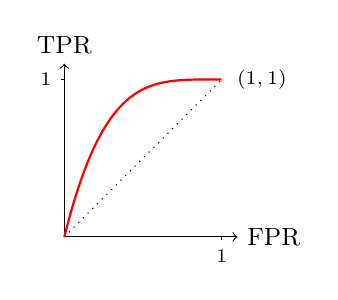
\begin{tikzpicture}[scale=2.0]
  \draw[->] (0,0) -- (1.1,0) node[right] {\small FPR};
  \draw[->] (0,0) -- (0,1.1) node[above] {\small TPR};
  \draw[dotted] (0,0) -- (1,1);
  \draw[smooth, thick, red] plot[domain=0:1] (\x, {1-(1-\x)*(1-\x)*(1-\x)*(1-\x)});
  \node at (1,1) [right=2pt] {\scriptsize $(1,1)$};
  \draw (0,1) -- (-0.02,1) node[left] {\scriptsize 1};
  \draw (1,0) -- (1,-0.02) node[below] {\scriptsize 1};
\end{tikzpicture}
\end{center}

\begin{enumerate}[(i)]
  \item \subpoints{1} What is plotted on the two axes of the ROC curve?
  \item \subpoints{1} Define the AUC and state what AUC $= 0.5$ corresponds to.
  \item \subpoints{1} The researcher proposes lowering the threshold from $0.5$ to $0.3$. How would you expect this to affect sensitivity and specificity, and where on the ROC curve does the operating point move?
\end{enumerate}

\subsection*{c) $K$-nearest neighbours \subpoints{4}}

A classmate fits a $K$-NN classifier with $K = 35$ on the same training data, using the predictors above (standardized). He produces the following test-set confusion matrix:

\begin{center}\small
\begin{tabular}{c|cc}
 & \textbf{Predicted: default} & \textbf{Predicted: no default} \\ \hline
\textbf{Actual: default}    & 200  & 400 \\
\textbf{Actual: no default} & 120  & 2280 \\
\end{tabular}
\end{center}

\begin{enumerate}[(i)]
  \item \subpoints{1} Briefly describe how a $K$-NN classifier produces a predicted class label for a new observation. (Two or three sentences.)
  \item \subpoints{2} Compute the sensitivity, specificity, and test error rate of this KNN classifier.
  \item \subpoints{1} The classmate did not standardize \texttt{balance} (measured in thousands) together with \texttt{pay\_0} (measured on a small integer scale). Why is this a problem for KNN, in particular?
\end{enumerate}

\subsection*{d) A tree-based competitor \subpoints{5}}

You want to fit a tree-based method to compete with the logistic regression. Choose one method we discussed in the course, and justify your choice.

\begin{enumerate}[(i)]
  \item \subpoints{2} State which tree-based method you would use (e.g.\ bagging, random forest, gradient boosting) and give a \emph{concrete numeric value} for each of its main tuning parameters (for a random forest, for instance: \texttt{mtry}, \texttt{ntree}, and the terminal-node size). \textbf{Justify each numeric choice} with one short sentence; a vague phrase like ``sufficiently many trees'' will not earn full credit.
  \item \subpoints{2} Suppose your chosen method gives test sensitivity $0.42$, test specificity $0.96$, and test error rate $0.14$. Compare to the logistic regression results from part (a). Which model would you prefer, and why? Make explicit which criterion drives your choice.
  \item \subpoints{1} Briefly describe what a \emph{variable-importance plot} from a random forest shows, and what kind of question it can (and cannot) answer.
\end{enumerate}

\subsection*{e) Class imbalance \subpoints{2}}

The marginal distribution of \texttt{default} on the full dataset is approximately
$$P(\texttt{default} = 1) \approx 0.20, \qquad P(\texttt{default} = 0) \approx 0.80.$$

\begin{enumerate}[(i)]
  \item \subpoints{1} A naive classifier that always predicts ``no default'' would already achieve a test error rate of approximately what value? Justify in one sentence.
  \item \subpoints{1} In light of (i), comment on whether \emph{test error rate} is the most appropriate metric for choosing between classifiers on this dataset. What metric or pair of metrics would you privilege instead, and why?
\end{enumerate}

\vspace{1em}
\hrule
\vspace{0.5em}

\noindent\textbf{End of exam.} \quad Total: $10 + 28 + 16 + 22 + 24 = 100$ points.

\end{document}
